\documentclass[11pt, oneside]{article}   	% use "amsart" instead of "article" for AMSLaTeX format
\usepackage{geometry}                		% See geometry.pdf to learn the layout options. There are lots.
\usepackage{textcomp}
\usepackage{hyperref}  % TODO: see page 94 of latex book
\geometry{letterpaper}                   		% ... or a4paper or a5paper or ... 
%\usepackage[parfill]{parskip}    		% Activate to begin paragraphs with an empty line rather than an indent
\usepackage{graphicx}				% Use pdf, png, jpg, or eps§ with pdflatex; use eps in DVI mode
								% TeX will automatically convert eps --> pdf in pdflatex		
\usepackage{amssymb}
\usepackage{amsmath}
\usepackage{relsize}

\title{CSCI 181 / E-181 Spring 2014 Practical 3 \\ 
{\large Kaggle Team "Capt. Jinglehiemer"}
}
\author{
  David Wihl\\
  \texttt{davidwihl@gmail.com}
  \and
  Zack Hendlin\\
  \texttt{zgh@mit.edu} 
}
%\date{}							% Activate to display a given date or no date

\begin{document}
\maketitle
\section*{Warm-Up}

We consider two approaches for classifying fruits (with length and width measurements provided) into one of three categories.

It is important to note that the data here is not perfectly linearly seperable, as can be seen in the plot below:

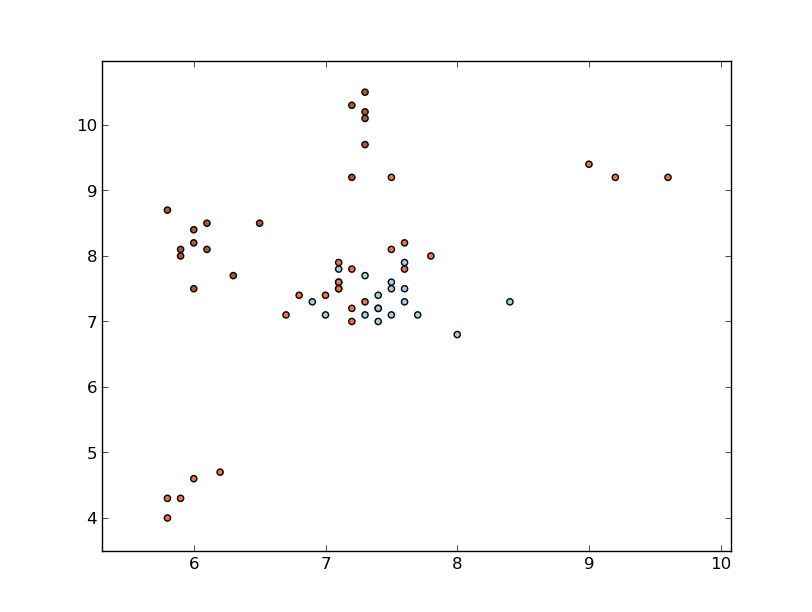
\includegraphics[scale=.6]{figure_3}

So the challenge becomes how we can best define mutually exclusive regions of the graph.

\subsection*{Logistic Classification}

Multiclass logistic classification seeks to define the weights that minimize:
\\
 $E(w_1, w_2, ..., w_K) =  -\sum\limits_{n=1}^N \sum\limits_{k=1}^K = t_{nk} ln_{nk}$ , 
as given in equation 4.108 in Bishop.
\
\\
Here our $w$ vector will have be $k x 3$ as we have a variable for height, weight, and then an offset term $w_0$.
\
\\
Since $k=3$, we fit 9 weights so as to minimize the error function. We use the Broyden Fletcher Goldfarb Shanno algorithm (BFGS) as implemented in the Scipy package. We select this because it provides a better approximation to the Hessian at each step.
\
\\
The error function achieves its minimum at 34.769598, and takes 44 iterations to converge.
\\
Once we have the weights:

\[
w=
  \begin{bmatrix}
    -7.35269067 & 2.48983592 & -1.17947522\\
    -3.65199071 & 1.66456348 & -0.81582258\\
    14.00478476 & -4.15564072 & 1.99410538\\	
	
  \end{bmatrix}
\]
\\
\
 we then use in the softmax function:
\
$y_k(\phi) = exp(a_k)/\sum\limits_{j=1}^K exp(a_j)$
\\
where $a$ is simply the dot product of $x$ and $w$,to evaluate which class has the highest likelihood for a particular data point. The point is then assigned to the class which has the highest class-conditional density.
\\
We get the resulting classification.

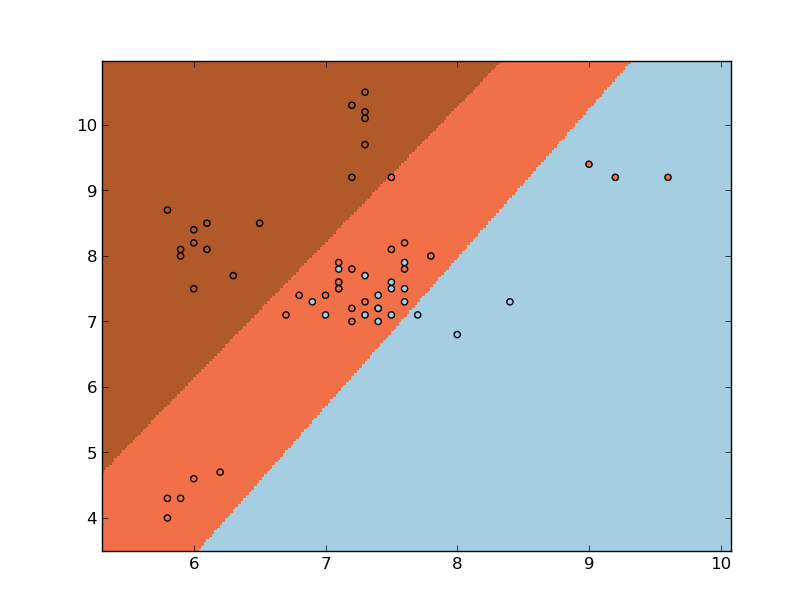
\includegraphics[scale=.6]{logistic_classifer}

\subsection*{Generative Model Classification}

Generative models attempt to determine, for each class $k$, a likelihood that a data point is generated by that particular class.
\\
\ We first calculate the prior likelihoods for each class $P(c_k)$
\\
\ And then recognizing we want $p(C_k |x_n)$ by applying Bayes rule, we need: $p(x_n |C_k)$.
\\
The multivariate normal is given by:
\
\\
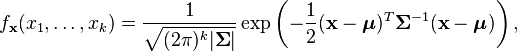
\includegraphics[scale=.5]{formula}
\
\\
where k=2 in our case because we have (1) height and (2) width.
\
\\
This gives us a probability density function for each class. We then apply Bayes rule:

$p(C_k |x_n) = p(x_n |C_k)  p(C_k) / \sum\limits_{j=1}^K p(x_n | c_j) * p(c_j)$

and note that we can ignore the denominator since it is the same for all classes.

\\
We then have an assignment for each point to the highest likelihood class as shown in plot below.
\\
\
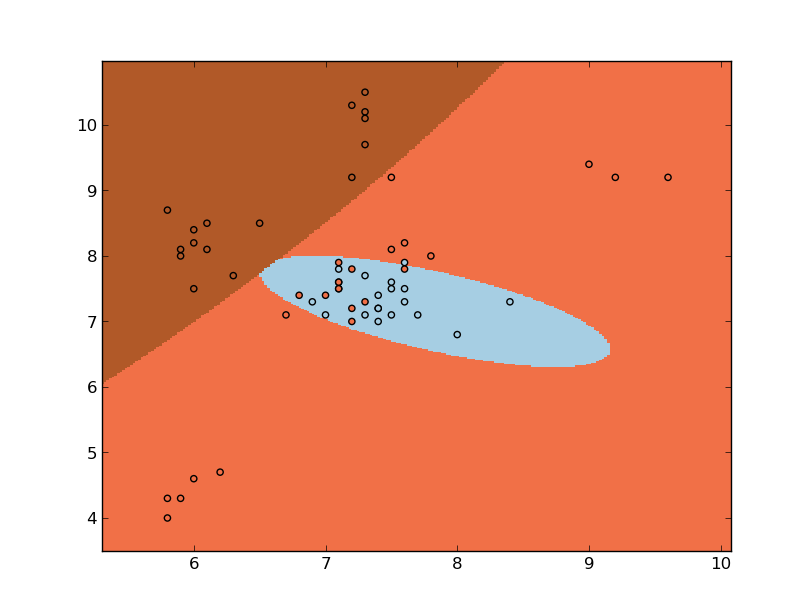
\includegraphics[scale=.6]{generative_classifier}


\subsection*{Warmup Summary}

As we can see from the graphs in the previos sections, allowing a non-linear decision boundry (as we did when we used the generative classifier) allowed more flexibility to capture clusters of points and indeed was more accurate at capturing the variation observed in the data.

\section*{Classifying Malicious Software}

\subsection*{Preliminary Data Analysis}

NOTES:
4GB of XML to parse and process, first step was to split the training and the testing. broke into vectorize, train and test steps, persisting appropriate intermediate data at each step. This also enabled parallelization of test runs over a cluster of machines.

\subsection*{Using Cross-validation}

Ran 5 CV sets of train / CV data 70/30, 80/20 and 90/10 for each classifier.

\section*{Approaches considered}

\subsection*{Feature Engineering}


Aggregate Features per training file:
 selected all process features  (e.g. 'startreason', 'terminationreason', 'username', 'executionstatus', 'applicationtype') and summary thread features (num of each type of system call).

used CV to generate Logistic Regression weights. Took mean and std of resulting matrix, then eliminated any features where abs(mean) $<$ 0.001 and std $< $0.01.



\subsection*{Selection of fitting technique}

Tried LogisticRegression and SVM with a number of different C values, none of which made a significant difference.

\subsection*{Exploratory Data Analysis}

\section*{Conclusion}

\end{document}  
